\section{Introducción}

Nos propusimos atacar el juego 4 en linea modificando la implementación del ta-te-ti.
Ambos juegos tienen similitudes, se gana logrando obtener una hilera, ya sea horizontal vertical o diagonal del mismo color.
Para el caso del ta-te-ti basta con alinear 3 fichas del mismo color, mientras que en el 4 en linea se necesitan 4, tal como su nombre
lo indica. Una diferencia importante, la cual impactó en la experimentación del trabajo,
es que el ta-te-ti se juega en un tablero de $3\times3$, mientras que el 4 en linea en uno de $7\times6$.
Debido a las similitudes y diferencias de los tipos de juego, decidimos plantear una serie de experimentos acordes a la capacidad de computo soportada
por nuestras computadoras.
%
% Primeros test:
%
% El algoritmo de \textbf{QLearning} utiliza los hiperparametros \textit{learning rate} y \textit{discount} y la inicializacion
%  de la matriz de valores de Q.
% Ademas necesitamos una politica de control, una cantidad de epocas para entrenar y un oponente contra quien jugar.
%
% En este punto empezamos a notar que tenemos una explosión combinatoria de parametros.
%
% Así que tomamos algunas decisiones:
%
% \begin{enumerate}
% \item La cantidad de epocas para entrenar serán 200.000
% \item La política de control que utilizaremos será \textbf{$\epsilon-greedy$}. Y tendremos que elegir el mejor $\epsilon$
% \item Nuestro oponente será random.
% \item Utilizaremos gridSearch para setear los valores de \textit{learning rate},  \textit{discount} y el valor con que
% inicializamos la matriz de Q. Estos tres parametros se moverán entre 0 y 1. Aumentado el valor de a 0.1
% \end{enumerate}
%
%
% El resultado fue que teniamos 14641 combinaciones distintas de parametros. Y correr esto
% era inviable por cuestiones de tiempo.
% Por este motivo decidimos fijar la inicializacion de la matriz de Q a 0. \textit{learning rate} y \textit{discount} a 0.5,
%  con la idea de tomar en cuenta por igual las recompensas futuras y las actuales. Y lo mismo con la informacion reciente y la pasada.
%
% Este recorte nos devolvía 11 combinaciones diferentes. Sin embargo el tiempo que tardaba en entrenar seguia siendo muy alto,
% motivo por el cual se nos ocurrió que en vez de jugar con un tablero de 7x6 y 4 en linea para ganar, podíamos escalarlo para
% ver si se comportaba de modo similar. Tomamos un tablero de 6x5 y 3 en linea para ganar.
%
%
% %La primer combinacion de parametros tardó aproximadamente 10 min en entrenar. Haciendo una proyeccion de cuanto podria tardar en total con todas las combinaciones tardaria aproximadamente 101 dias, otra señal de que teniamos que reducir la cantidad de combinaciones.
%
%
% Asi variamos los diferentes epsilons y obtuvimos que el jugador QLearning ganó el 91\% de las veces con los
% siguientes parametros: \\
%
% \begin{itemize}
%   \item  \textbf{$\epsilon$} = 0.0
%   \item \textbf{learning\_rate} = 0.5
%   \item \textbf{discount} = 0.5
%   \item \textbf{initialQ} = 0.0
% \end{itemize}
%
%
% %(0.911855, {'discount': 0.5, 'learning_rate': 0.5, 'initialQ': 0.0, 'epsilon': 0.0})
%
% En la siguiente prueba fijamos el valor de epsilon al mejor resultado 0 y movimos learning\_rate del mismo modo.
% Obteniendo que con 0.9 ganaba el 95\% de las veces. Luego fijamos learning\_rate a 0.9 e hicimos lo mismo con discount y
% gano 3l 93\% de las veces con 0.1. \\
%
% Solo nos restaba probar que pasaba con la inicialización de la matriz Q. Decidimos tomar los mejores resultados del paso
%  anterior e inicializarla con valores entre 0 y 1. Aumentado el paso en 0.1. Y tambien probar que pasaba si inicializabamos
%  todos los valores random. \\
%
% El mejor valor obtenido fue para la inicializacion con el valor 0. Y gano el  el 93\% de las veces. La mejor combinación que
%  obtuvimos fué:
%
% \begin{itemize}
%   \item  \textbf{$\epsilon$} = 0.0
%   \item \textbf{learning\_rate} = 0.9
%   \item \textbf{discount} = 0.5
%   \item \textbf{initialQ} = 0.0
% \end{itemize}
%
%
%
% Lo que podemos observar es que:
% \begin{itemize}
%   \item  Darle mucho peso a la información reciente da buenos resultados.
%   \item  Es tan importante tomar en cuenta las recompesas actuales como las futuras.
%   \item  Siempre explotar la informacion que ya conocemos, nunca explorar.
%   \item  Es mejor no asignarle ningun valor arbitrario a la matriz de Q. Mejor ir aprendiendo los valores en funcion de
%    los juegos.
%
% \end{itemize}
%
% %\begin{frame}
% \begin{figure}[h]
%  \centering
%   \begin{minipage}[c]{1\textwidth}
% 	\centering
% 	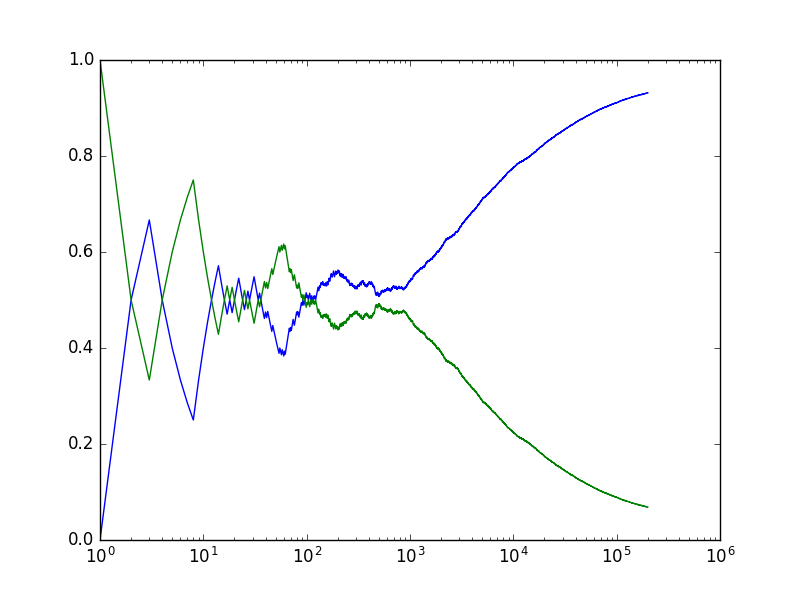
\includegraphics[scale=0.5]{img/QlearningRandomEgreedy200000.png}
%         \caption{Qlearning vs Random 200000 juegos}
%   \end{minipage}
% \end{figure}
% %\end{frame}
%
% Lo que podemos observar es que efectivamente el jugador QLearning aprende, pues a medida que aumenta la cantidad de juegos
%  gana mayor cantidad de partidas. Contrariamente al jugador random.  \\
%
% Que pasa si jugabamos contra otro jugador Q-learning, bajo la combinación de paramtros obtenida en el paso anterior?.
%  Suponemos que en algún momento empezarán a empatar porque ambos aprendieron a jugar.\\
%
% \begin{figure}[h]
%  \centering
%  \begin{minipage}{.45\textwidth}
%   %\begin{minipage}[c]{1\textwidth}
% 	\centering
% 	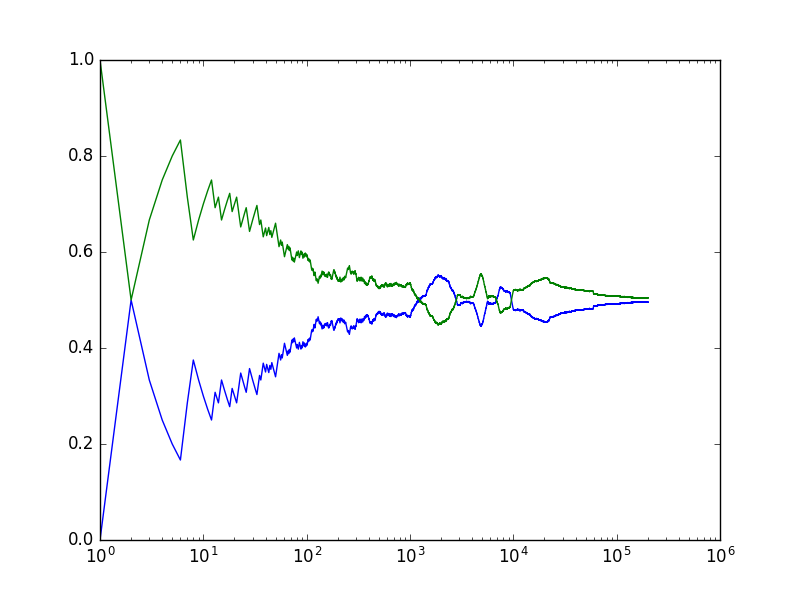
\includegraphics[scale=0.35]{img/QlearningQlearningEgreedy200000.png}
%         \caption{Qlearning vs Qlearning 200000 juegos}
%   \end{minipage}
%  \begin{minipage}{.5\textwidth}
% 	\centering
% 	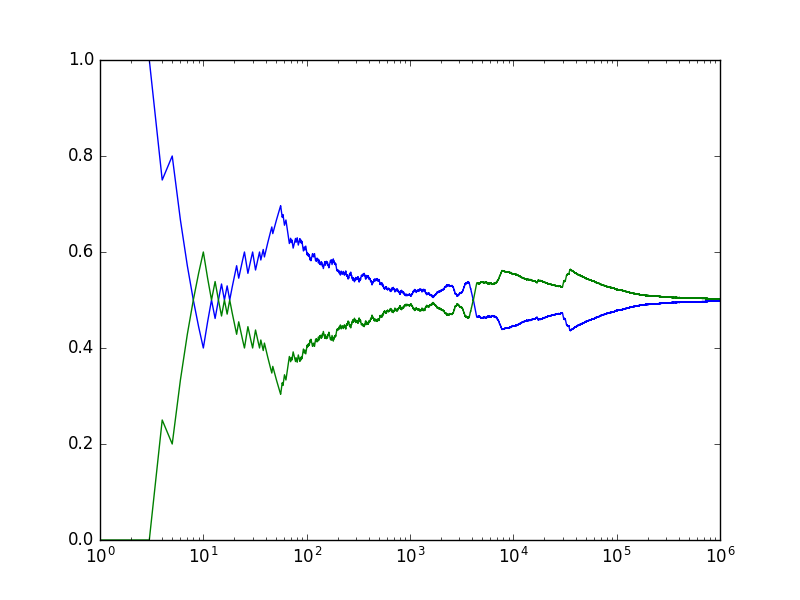
\includegraphics[scale=0.35]{img/QlearningQlearningEgreedy1000000.png}
%         \caption{Qlearning vs Qlearning 1000000 juegos}
%   \end{minipage}
% \end{figure}
%
%
% \begin{figure}[h]
%  \centering
%  \begin{minipage}{.45\textwidth}
%   %\begin{minipage}[c]{1\textwidth}
% 	\centering
% 	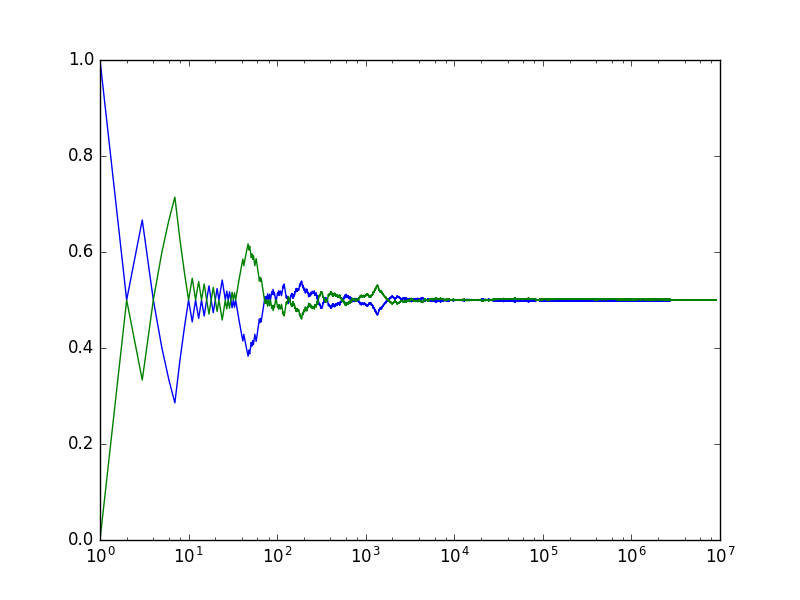
\includegraphics[scale=0.35]{img/QlearningQlearningEgreedy9000000.png}
%         \caption{Qlearning vs Qlearning 9000000 juegos}
%   \end{minipage}
% \end{figure}
%
%
% Podemos ver como a la hora de enfrentarse contra otro jugador, que tambien aprende, llega un momento donde se estabiliza la
%  cantidad de veces que gana cada uno. Esto no se corresponde con la idea que teniamos. \\
%
% Asi que decidimos jugar contra el jugador Q-learning entrenado para ver como estaba jugando. Y lo que notamos es que cuando comienza
%  a jugar, siempre tiene una estrategia ganadora.\\
% {\huge EXPLICAR BIEN LA ESTRATEGIA GANADORA}\\
%
% Y esto explicaría porque no empatan. Como el jugador que comienza tiene una estrategia ganadora siempre va a ganar.\\
%
%
% Sin embargo estamos jugando un juego con un tablero de dimension menor, asi que queremos ver que pasa si entrenamos con los mismos
%  parametros y las caracteriticas del juego original.
%
% \begin{figure}[h]
%  \centering
%   \begin{minipage}[c]{1\textwidth}
% 	\centering
% 	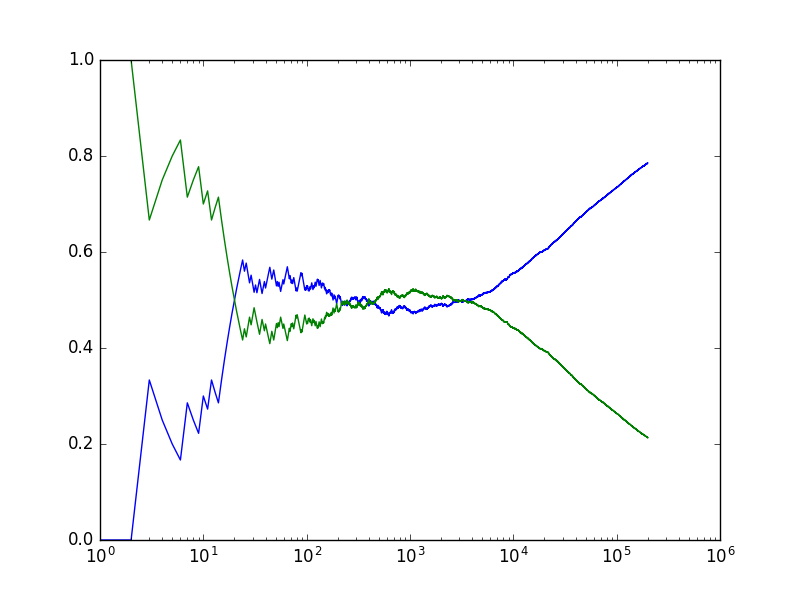
\includegraphics[scale=0.5]{img/QlearningRandomEgreedy2000007x6(4).png}
%         \caption{Qlearning vs Random 200000 juegos}
%   \end{minipage}
% \end{figure}
%
% Lo que podemos observar es bastante razonable, como agrandamos el tablero tenemos muchas mas combinaciones, motivo por el cual,
%  tarda mas tiempo en aprender como ganar.
%
% En este caso ya no encontramos estrategia ganadora para los mismos parametros.
% {\huge EXPLICAR MEJOR ESTO}\\
%
%
% \begin{figure}[h]
%  \centering
%  \begin{minipage}{.45\textwidth}
% 	\centering
% 	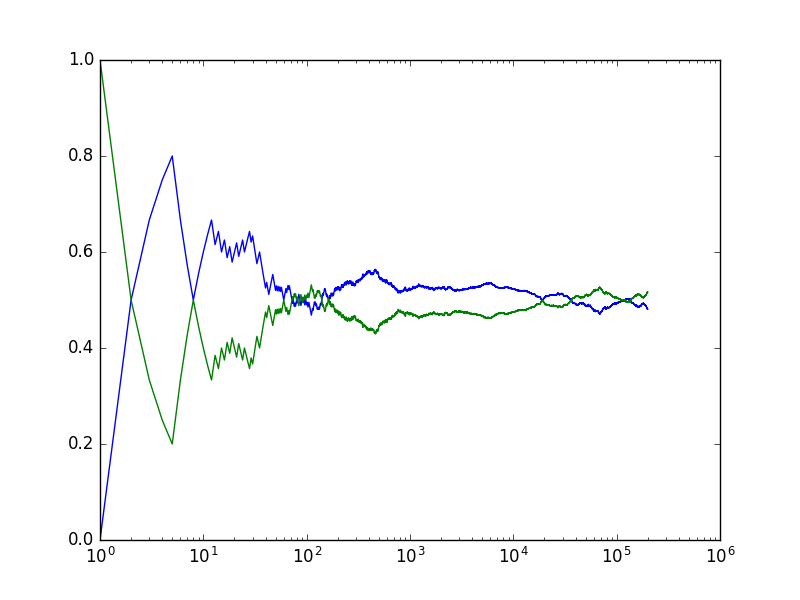
\includegraphics[scale=0.35]{img/QlearningQlearningEgreedy2000007x6(4).png}
%        \caption{Qlearning vs Qlearning 200000 juegos}
%   \end{minipage}
% % \begin{minipage}{.5\textwidth}
% %	\centering
% %	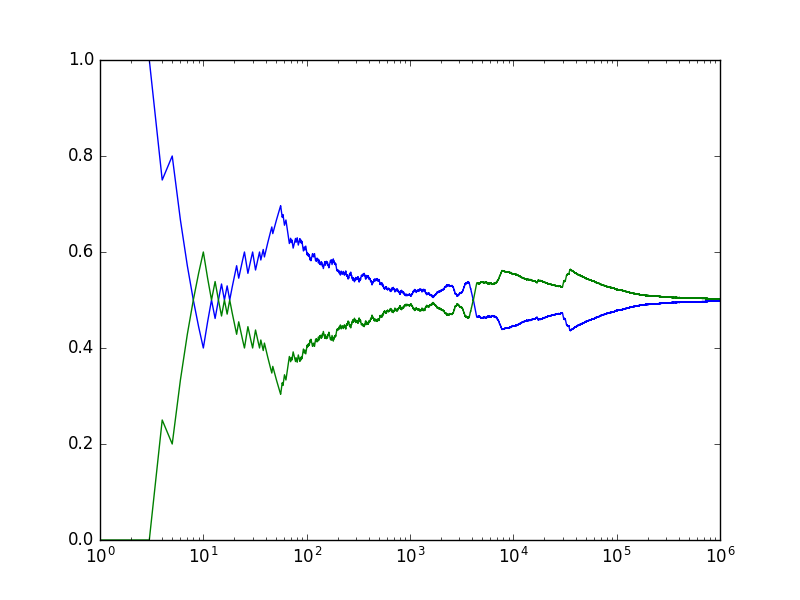
\includegraphics[scale=0.35]{img/QlearningQlearningEgreedy1000000.png}
% %        \caption{Qlearning vs Qlearning 1000000 juegos}
% %  \end{minipage}
% \end{figure}
%
% No pudimos probar Qlearning Vs Qlearning con 9000000 juegos debido al tiempo de computo.
%
%
% Asi que pensamos en probar otra politica de control softmax.
%
% Otra vez nos dimos a la tarea de buscar los parametros. En este caso necesitamos definir un tau y una funcion de decremento
%  ademas de textit{learning rate}, \textit{discount}, cantidad de epocas, y los valores de inicializacion de Q. Para estos ultimos exploramos valores que se encontraban alrededor de los encontrados para la estrategia e-greedy.
% Empezamos con el tabler de 6x5 y 3 fichas y una vez encontrado los parametros pasamos al tablero real.
%
%
